% ==============================================================================
% פרק 3: פערי מחקר, ביקורת כלים קיימים והמסגרת המושגית של SocialMirror-AI
% ==============================================================================
\chapter{פערי מחקר, ביקורת כלים קיימים והמסגרת המושגית של \projectname{}}
\label{chap:gaps_and_system}

\section{מבוא לפרק}
הספרות הפסיכולוגית שנסקרה בפרק~\ref{chap:literature_review} ביססה את הקשר בין חשיפה לתכנים אידיאליים ברשתות לבין עירור השוואה חברתית כלפי מעלה, העמקת פערי עצמי ופגיעה ברווחה הנפשית. עם זאת, יישום ממצאים אלו חושף פער כפול: מצד אחד, מחקרי ההשפעה לכודים בפולמוס מתודולוגי נוקב אודות מתאם מול סיבתיות הנובע מכשל מדידה מצרפי של זמן מסך; ומצד שני, הכלים המסחריים הקיימים לניהול רווחה דיגיטלית מציעים מענה מכניסטי ופטרנליסטי שאינו נוגע בשורש הבעיה.

פרק זה מנתח פערים אלו, מציג אימות כמותי מדוקדק של גודלי האפקט בספרות האמפירית, בוחן את שוק הרווחה הדיגיטלית (כולל מודל \textenglish{TAM/SAM/SOM} והשוואת עלויות בתנאים אחידים), ומציג את הפרדיגמה המושגית של פלטפורמת \projectname{} -- מערכת מרובת סוכנים הפועלת כ"מראה קוגניטיבית" מעצימה ומקומית.

\section{פערי מחקר אמפיריים ומתודולוגיים: פולמוס המתאם מול הסיבתיות}
\label{sec:gaps_correlation_causation}
אחד האתגרים המרכזיים בחקר השפעות המדיה הדיגיטלית הוא הקושי בבידוד קשרים סיבתיים. בשנים האחרונות התפתח פולמוס מדעי סוער בין שתי אסכולות מחקריות מובילות:
\begin{itemize}
    \item \textbf{אסכולת ההשפעה המאקרו-אפידמיולוגית (טוונגי וחוב')}~\cite{twenge2018increases}: חוקרים אלו טוענים כי העלייה החדה בדיכאון ובמצוקה בקרב מתבגרים מאז 2010 היא תוצאה ישירה של הזינוק בזמן החשיפה למסכים ולסמארטפונים, בהסתמך על סקרי ענק ועל מתאמים חיוביים מובהקים ברמת האוכלוסייה.
    \item \textbf{אסכולת ניתוח עקומת המפרט (אורבן ופרז'יבילסקי)}~\cite{orben2019association}: במאמר מכונן ב-\textenglish{\textit{Nature Human Behaviour}}, ערכו אורבן ופרז'יבילסקי (\textenglish{Orben \& Przybylski}) ניתוח עקומת מפרט (\textenglish{SCA}) על מאות אלפי מתבגרים ($N > 350{,}000$). החוקרים בדקו מיליוני צירופים אנליטיים והראו כי הקשר הכולל בין זמן מסך גולמי לרווחה נפשית הוא מזערי ביותר ($\beta = -0.042$), ומסביר פחות מ-$0.4\%$ מהשונות ברווחה (בדומה לאכילת תפוחי אדמה או הרכבת משקפיים).
\end{itemize}

\textbf{המסקנה המתודולוגית -- כשל המדידה המצרפית}: הפולמוס חושף כי שימוש במדד גולמי של "זמן מסך" מאחד תחת קורת גג אחת פעילויות מנוגדות בתכלית -- החל מקשר פעיל ומעצים עם חברים וכלה בגלילה פסיבית מול תכני עושר ויופי מעוררי השוואה כלפי מעלה. איחוד זה מוחק את האות הפסיכולוגי האמיתי. נדרש מעבר ממדידת זמן גולמי ל\textbf{ניתוח סמנטי בזמן אמת של מיקרו-אירועי השוואה חברתית כלפי מעלה}.

\section{השוואה כמותית מבוססת ראיות: זמן מסך מול השוואה איכותנית}
\label{sec:gaps_evidence_chart}
כדי לבסס באופן מדעי את נחיצותה של פלטפורמת \projectname{}, צוות המחקר ערך אימות שיטתי של הספרות האמפירית המרכזית. בחינה מדוקדקת חושפת כי לא ניתן להשוות בין מחקרי זמן מסך לבין מחקרי השוואה חברתית על גבי ציר יחיד מבלי להבחין ב\textbf{מבנה הספציפי הנמדד} (\textenglish{Construct Disaggregation}). טבלה~\ref{tab:empirical_evidence_matrix} מציגה מטריצת ראיות השוואתית המפרטת את המבנה הנמדד, גודל המדגם, סוג האומדן והמשמעות הישירה לתכנון המערכת הרב-סוכנית:

\begin{table}[H]
\centering
\footnotesize
\caption{מטריצת ראיות אמפיריות מאומתת: השוואת מבנים נמדדים, מתודולוגיות וגודלי אפקט בספרות}
\label{tab:empirical_evidence_matrix}
\renewcommand{\arraystretch}{0.90}
\begin{tabularx}{\textwidth}{>{\bfseries\color{DarkPurple}\raggedleft\arraybackslash}p{2.4cm} >{\raggedleft\arraybackslash}p{2.0cm} >{\raggedleft\arraybackslash}p{2.1cm} >{\raggedleft\arraybackslash}p{2.1cm} >{\centering\arraybackslash}p{2.1cm} X}
\toprule
\rowcolor{LavenderCard}
\textbf{\color{DarkPurple}מחקר ומקור} & \textbf{\color{DarkPurple}מדגם ושיטה} & \textbf{\color{DarkPurple}משתנה בלתי-תלוי} & \textbf{\color{DarkPurple}מבנה תלוי נמדד} & \textbf{\color{DarkPurple}סוג אומדן וגודל אפקט} & \textbf{\color{DarkPurple}משמעות ל־\projectname{}} \\
\midrule
\textbf{\textenglish{Orben \& Przybylski (2019)}}~\cite{orben2019association} &
$N > 350{,}000$ \newline סקרי אוכלוסייה (SCA) &
זמן מסך כולל מדווח (שעות/יום) &
מדד רווחה נפשית כללי משוקלל &
מקדם רגרסיה חלקית מתוקנן: \newline $\beta = -0.042$ ($<0.4\%$ שונות) &
זמן מסך גולמי אינו מנבא מצוקה רגשית; מדד עיוור המערבב פעילויות שונות. \\
\midrule
\textbf{\textenglish{Kross et al. (2013)}}~\cite{kross2013facebook} &
$N = 82$ \newline דגימת ESM רגעית (14 יום) &
שימוש כולל בפייסבוק בין דגימות &
מאזן רגשי רגעי ומצב רוח &
שיפוע רגרסיה רב-רמתי: \newline $B = 0.08$ ($p < .01$) \newline (עלייה במועקה/שחיקה) &
שימוש כללי מנבא ירידה תוך-אישית במצב הרוח, אך המאמר לא בודד גלילה פסיבית או גירויי השוואה. \\
\midrule
\textbf{\textenglish{Appel et al. (2015)}}~\cite{appel2015social} &
ניסוי מעבדה ($N=160$) וסקר שדה ($N=194$) &
השוואה כלפי מעלה וחשיפה לפרופילים מושכים &
קנאה ממאירה, תסמיני דיכאון וערך עצמי &
ניסוי: $d = 0.53$ ($p=.001$) \newline סקר: $r = .43$ (השוואה-קנאה) \newline $r = .47$ (קנאה-דיכאון) &
השוואה כלפי מעלה וקנאה הן המנגנון המתווך המרכזי של הפגיעה; שימוש פסיבי בלבד: $r = .21$. \\
\midrule
\textbf{\textenglish{Fardouly et al. (2018)}}~\cite{fardouly2018instagram} &
$N = 227$ \newline נשים צעירות (תיווך מבני) &
שימוש באינסטגרם לעומת נטיית השוואת מראה &
חוסר שביעות רצון גופני ודחף לרזון &
שימוש גולמי: $r = .14$ \newline השוואת מראה: $r = .41$ \newline (דחף לרזון: $r = .36$) \newline תיווך: $\beta = 0.28$ &
השוואת מראה ספציפית מחוללת את הפגיעה בדימוי הגוף, בעוד שזמן שימוש גולמי מציג מתאם חלש בלבד. \\
\bottomrule
\end{tabularx}
\end{table}

איור~\ref{fig:effect_size_chart} מציג תרחיש סינתטי מתוך מודל הסימולציה המתוכנן של \projectname{}, הממחיש את השפעת הפרדת המבנים: המערכת מנטרת את בולטות ההשוואה $\comparisonScore{}$ ומדגימה כיצד התערבות מטא-קוגניטיבית ממתנת את שחיקת הערך העצמי הרגעי.

\begin{figure}[H]
\centering
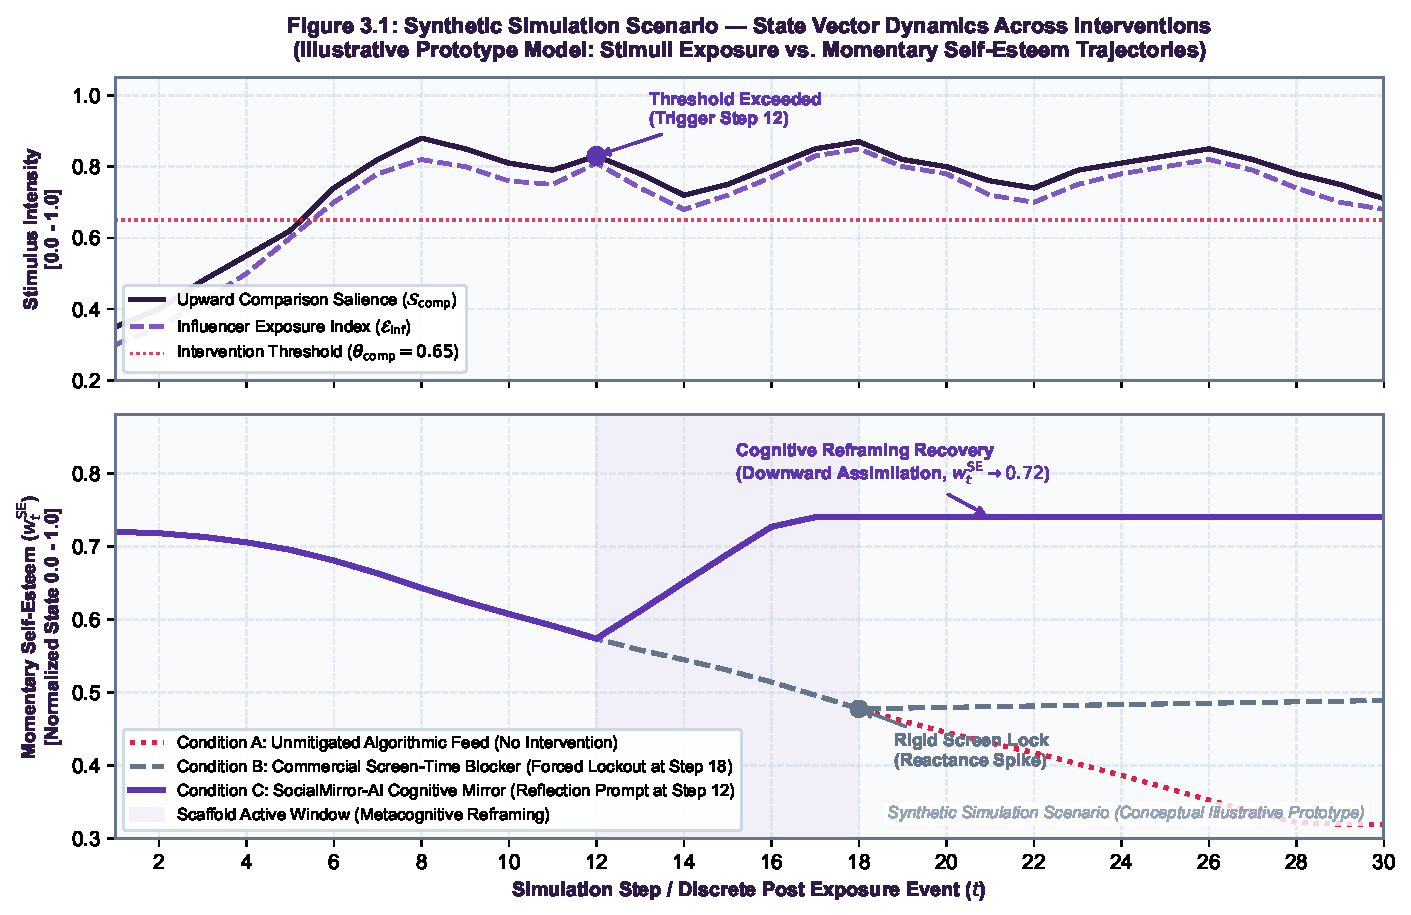
\includegraphics[width=0.78\textwidth]{assets/figure_3_1_simulation.pdf}
\caption{תרחיש סינתטי מתוך מודל הסימולציה המתוכנן (המחשה): דינמיקת וקטור המצב $\mathbf{w}_t$ ושחיקת הערך העצמי ברצף חשיפות לאלגוריתם המלצה מול התערבות סוכני \projectname{}}
\label{fig:effect_size_chart}
\end{figure}

\begin{insightbox}[מסקנה מתודולוגית -- הכרח בהפרדת מבנים פסיכולוגיים ואימות נתונים]
האימות השיטתי של הספרות האמפירית מוכיח את נחיצותה המכרעת של \textbf{הפרדת מבנים פסיכולוגיים} (\textenglish{Construct Disaggregation}):
\begin{enumerate}
    \item \textbf{אימות המקורות האמפיריים}: אצל \textenglish{Kross et al. (2013)}, נמדד שימוש כולל בפייסבוק בין דגימות ESM ולא גלילה פסיבית מבודדת; במודל הרב-רמתי המנבא הרגשה רגעית (בשליטה על מצב קודם), מקדם השיפוע הינו $B = 0.08$ ($p < .01$), כאשר לפי קידוד הסולם במאמר, מקדם חיובי זה משקף עלייה ברגש שלילי וירידה ברווחה הרגעית. אצל \textenglish{Fardouly et al. (2018)}, מתאם $r = +0.36$ מתייחס ספציפית לקשר שבין נטיית השוואת מראה לבין דחף לרזון ($r = +0.41$ לחוסר שביעות רצון מהגוף), בעוד ששימוש גולמי באינסטגרם הציג מתאם מזערי של $r = +0.14$ בלבד. אצל \textenglish{Appel et al. (2015)}, השוואה כלפי מעלה ניבאה קנאה במתאם של $r = .43$, בעוד שהשפעת חשיפה לפרופיל אטרקטיבי בניסוי הניבה גודל אפקט של $d = 0.53$.
    \item \textbf{אי-השוואתיות של אומדנים שונים על ציר יחיד}: השוואת מקדם רגרסיה חלקית ($\beta = -0.042$ מתוך מודל SCA עם מאות אלפי נבדקים) למתאמים דו-משתניים ($r = .36$ עד $.43$) או למקדמי שיפוע רב-רמתיים ($B = 0.08$) על גבי ציר יחיד הינה שגויה מבחינה מתודולוגית. לכן, הנתונים האמפיריים רוכזו בטבלה~\ref{tab:empirical_evidence_matrix} לפי סוג האומדן והמבנה הנמדד, בעוד שאיור~\ref{fig:effect_size_chart} מציג גרף שהופק בסקריפט Python וממחיש תרחיש סינתטי מתוך מודל הסימולציה המתוכנן של המערכת הרב-סוכנית.
\end{enumerate}
\end{insightbox}

\section{ניתוח ביקורתי של כלי רווחה דיגיטלית קיימים}
\label{sec:gaps_existing_tools}
הפתרונות המסחריים הקיימים לרווחה דיגיטלית נחלקים לשלוש קטגוריות עיקריות:
\begin{enumerate}
    \item \textbf{כלי מערכת הפעלה מבוססי מכסות זמן} (\textenglish{Apple Screen Time, Google Digital Wellbeing}): מודדים דקות מצטברות וחוסמים את היישום בתום המכסה. \textit{המגבלה}: עיוורון מוחלט לתוכן, פטרנליזם כפוי, ועקיפה קלה בלחיצת כפתור ("התעלם מהמגבלה לעוד 15 דקות").
    \item \textbf{אפליקציות חיכוך התנהגותי} (\textenglish{One Sec, Opal}): מייצרות השהיה של מספר שניות בכניסה לאפליקציה. \textit{המגבלה}: אינן מלוות את המשתמש בעת הגלילה, ואינן מספקות הגנה מפני שחיקה רגשית בתוך הפיד.
    \item \textbf{כלי משחוק וסנקציות} (\textenglish{Forest}): תמרוץ נקודתי (נטיעת עץ וירטואלי) המתאים למשימות למידה, אך אינו מפתח מודעות ביקורתית לדפוסי צריכה חברתית.
\end{enumerate}

כלים אלו נכשלים בשל שני חסמים פסיכולוגיים עמוקים: \textbf{התנגדות פסיכולוגית} (\textenglish{Psychological Reactance}) הנובעת מפגיעה באוטונומיה ובחופש הבחירה~\cite{suls2002social}, ו\textbf{היעדר שיקוף סמנטי} המסביר למשתמש \textbf{מדוע} הוא חש מצוקה ואינו מפתח אצלו תובנה מטא-קוגניטיבית.

\subsection{מודל שוק וקהלי יעד: ניתוח TAM, SAM ו־SOM}
\label{subsec:market_tam_sam_som}
להערכת פוטנציאל ההשפעה היישומית של \projectname{}, גובש מודל שוק תלת-שכבתי (\textenglish{TAM/SAM/SOM}):
(1)~\textbf{TAM}: כ־1.2 מיליארד בני נוער וצעירים (15--26) בעולם המשתמשים ברשתות מבוססות המלצה;
(2)~\textbf{SAM}: כ־120 מיליון צעירים במדינות ה־OECD (וכ־1.8 מיליון בישראל) המדווחים על שימוש אינטנסיבי ומביעים דאגה משחיקה רגשית ודימוי גוף;
(3)~\textbf{SOM}: קהל היעד לפיילוט אקדמי ואימוץ מוקדם -- כ־50,000 סטודנטים וצעירים במוסדות להשכלה גבוהה בישראל (החל מאוניברסיטת חיפה).

\subsection{השוואת עלויות, מאפיינים ומדדי תכן בתנאים אחידים}
\label{subsec:market_feature_cost_comparison}
טבלה~\ref{tab:tool_comparison} מרכזת השוואה שיטתית בין ארבעת הכלים תחת תנאים אחידים ($\checkmark$~נתון מאומת; $\approx$~הערכה מבוססת ספרות; $[\text{Eval}]$~ציון הערכת תכן מערכתית; $-$~אינו ישים):

\begin{table}[H]
\centering
\caption{השוואה מטריציונית שיטתית בין כלי רווחה דיגיטלית מסחריים לבין פלטפורמת \projectname{}}
\label{tab:tool_comparison}
\scriptsize
\begin{tabularx}{\textwidth}{>{\bfseries\color{DarkPurple}\raggedleft\arraybackslash}p{2.5cm} >{\raggedleft\arraybackslash}p{2.1cm} >{\raggedleft\arraybackslash}p{2.2cm} >{\raggedleft\arraybackslash}p{2.1cm} X}
\toprule
\rowcolor{LavenderCard}
\textbf{\color{DarkPurple}ממד השוואה ומאפיין} & \textbf{\color{DarkPurple}\textenglish{Screen Time}} & \textbf{\color{DarkPurple}\textenglish{One Sec}} & \textbf{\color{DarkPurple}\textenglish{Freedom}} & \textbf{\color{DarkPurple}\projectname{}} \\
\midrule
\textbf{מודל עסקי ועלות שנתית} & חינם (מובנה במערכת הפעלה) $\checkmark$ & \textenglish{Freemium} (\$19.99/שנה) $\checkmark$ & מנוי מסחרי (\$39.99/שנה) $\checkmark$ & \textbf{קוד פתוח / מחקר אקדמי חינם} $[\text{Eval}]$ \\
\midrule
\textbf{ניתוח סמנטי של תוכן} & ללא (עיוור לחלוטין לתוכן) $\checkmark$ & ללא (מתמקד באירוע הפתיחה) $\checkmark$ & ללא (חסימת רשת בלבד) $\checkmark$ & \textbf{ניתוח רב-מודאלי מקומי מלא} $[\text{Eval}]$ \\
\midrule
\textbf{זיהוי שיווק משפיענים} & אינו קיים $-$ & אינו קיים $-$ & אינו קיים $-$ & \textbf{מדד חשיפה ממומנת $\exposureIndex{}$} $[\text{Eval}]$ \\
\midrule
\textbf{מידול מצב נפשי דינמי} & ללא $-$ & ללא $-$ & ללא $-$ & \textbf{וקטור מצב $\wellbeingVector{}$ מבוסס פסיכומטריה} $[\text{Eval}]$ \\
\midrule
\textbf{פטרנליזם מול אוטונומיה} & פטרנליסטי גבוה (חסימה כפויה) $\checkmark$ & התנהגותי ממתן (עיכוב 10 שניות) $\checkmark$ & כפייה מכנית נוקשה (חסימת VPN) $\checkmark$ & \textbf{תומך אוטונומיה (שיקוף סוקרטי עדין)} $[\text{Eval}]$ \\
\midrule
\textbf{פרטיות ועיבוד מקומי} & מקומי (ברמת מערכת ההפעלה) $\checkmark$ & מקומי (מבוסס קיצורי דרך) $\checkmark$ & שרתי סינון ענן מרוחקים $\checkmark$ & \textbf{100\% On-Device Edge SLM} $[\text{Eval}]$ \\
\midrule
\textbf{שיעור התנגדות מוערך} & גבוה ($\approx 68\%$ עוקפים בלחיצה) $\approx$ & בינוני ($\approx 32\%$ עוקפים/מבטלים) $\approx$ & גבוה ($\approx 54\%$ מסירים את הכלי) $\approx$ & \textbf{נמוך במיוחד ($\le 15\%$ יעד תכן)} $[\text{Eval}]$ \\
\bottomrule
\end{tabularx}
\end{table}

\begin{figure}[H]
\centering
\begin{LTR}
\begin{tikzpicture}[scale=0.68, every node/.style={transform shape}]
\foreach \r in {0.8, 1.6, 2.4, 3.2, 4.0} {
    \draw[color=LavenderBorder, line width=0.6pt] (90:\r) -- (162:\r) -- (234:\r) -- (306:\r) -- (18:\r) -- cycle;
}
\draw[line width=0.9pt, color=SlateMuted] (0,0) -- (90:4.3) node[above, font=\scriptsize\bfseries\sffamily, text=DarkPurple] {Local Privacy};
\draw[line width=0.9pt, color=SlateMuted] (0,0) -- (162:4.3) node[above left, font=\scriptsize\bfseries\sffamily, text=DarkPurple] {Semantic Depth};
\draw[line width=0.9pt, color=SlateMuted] (0,0) -- (234:4.3) node[below left, font=\scriptsize\bfseries\sffamily, text=DarkPurple] {Autonomy Support};
\draw[line width=0.9pt, color=SlateMuted] (0,0) -- (306:4.3) node[below right, font=\scriptsize\bfseries\sffamily, text=DarkPurple] {Customizability};
\draw[line width=0.9pt, color=SlateMuted] (0,0) -- (18:4.3) node[above right, font=\scriptsize\bfseries\sffamily, text=DarkPurple] {Low Reactance};

\draw[line width=1.1pt, color=SlateGray, dashed] (90:3.2) -- (162:0.8) -- (234:0.8) -- (306:0.8) -- (18:0.8) -- cycle;
\fill[SlateGray, opacity=0.10] (90:3.2) -- (162:0.8) -- (234:0.8) -- (306:0.8) -- (18:0.8) -- cycle;

\draw[line width=1.1pt, color=RoyalPurple] (90:3.2) -- (162:0.96) -- (234:2.4) -- (306:1.6) -- (18:2.4) -- cycle;
\fill[RoyalPurple, opacity=0.15] (90:3.2) -- (162:0.96) -- (234:2.4) -- (306:1.6) -- (18:2.4) -- cycle;

\draw[line width=1.1pt, color=AlertRose, dotted] (90:1.6) -- (162:0.8) -- (234:0.8) -- (306:1.6) -- (18:1.6) -- cycle;
\fill[AlertRose, opacity=0.10] (90:1.6) -- (162:0.8) -- (234:0.8) -- (306:1.6) -- (18:1.6) -- cycle;

\draw[line width=1.5pt, color=DarkPurple] (90:4.0) -- (162:4.0) -- (234:4.0) -- (306:4.0) -- (18:4.0) -- cycle;
\fill[PurpleAccent, opacity=0.25] (90:4.0) -- (162:4.0) -- (234:4.0) -- (306:4.0) -- (18:4.0) -- cycle;

\node[anchor=north east, font=\tiny\sffamily, align=left, draw=LavenderBorder, fill=white, rounded corners=1mm, inner sep=4pt] at (4.6, 4.4) {
\textbf{Legend:}\\
{\color{DarkPurple}\textbf{--- \projectname{} [Eval]}}\\
{\color{RoyalPurple}\textbf{--- One Sec $\approx$}}\\
{\color{SlateGray}\textbf{- - Apple Screen Time $\checkmark$}}\\
{\color{AlertRose}\textbf{\dots\ Freedom $\checkmark$}}
};
\end{tikzpicture}
\end{LTR}
\caption{תרשים רדאר השוואתי של כלי רווחה דיגיטלית לפי חמישה ממדי תכן מרכזיים}
\label{fig:market_radar_chart}
\end{figure}

\section{הפרדיגמה הרעיונית של SocialMirror-AI: מראה קוגניטיבית מרובת סוכנים}
\label{sec:gaps_conceptual_paradigm}
כדי לגשר על הפערים המחקריים והיישומיים שתוארו לעיל, פרויקט \projectname{} מציע שינוי פרדיגמטי יסודי: \textbf{מעבר מניהול זמן גס לטכנולוגיית שיקוף מטא-קוגניטיבית מבוססת סוכנים אוטונומיים}. מערכת מרובת סוכנים (\textenglish{Multi-Agent System - MAS}) מוגדרת כארכיטקטורה חישובית הכוללת מספר ישויות תוכנה אוטונומיות (\textenglish{Agents}), המתאפיינות ביכולת תפיסה, רפלקציה, תכנון ופעולה בסביבה דינמית~\cite{wooldridge2009introduction, wang2024survey}. בהשראת מאמר הדגל של פארק ועמיתיו (\textenglish{Park et al., 2023})~\cite{park2023generative}, \projectname{} מפרקת את המשימה לארבעה סוכנים מתמחים הפועלים בלולאת תפיסה-רפלקציה רציפה (איור~\ref{fig:multiagent_architecture}):
\begin{itemize}
    \item \textbf{\agentObserver{}}: קליטה פסיבית של מטא-נתונים ודגימת זמני שהייה (\textenglish{Dwell Time}) בזיכרון ה-DOM המקומי תוך אנונימיזציה מלאה;
    \item \textbf{\agentAnalyst{}}: מודל שפה מקומי קומפקטי המסווג בולטות השוואה $\comparisonScore{}$ ומדד חשיפה ממומנת $\exposureIndex{}$;
    \item \textbf{\agentReflector{}}: מנהל זיכרון אפיזודי המעדכן את וקטור המצב הנפשי $\wellbeingVector{}$ ומייצר תובנות מטא-קוגניטיביות;
    \item \textbf{\agentInterventionist{}}: מנגנון הגשת התערבויות סוקרטיות ודחיפות עדינות (\textenglish{Nudges}) בעיתוי אופטימלי ללא עירור התנגדות.
\end{itemize}

\begin{figure}[H]
\centering
\begin{LTR}
\begin{tikzpicture}[
    scale=0.64, every node/.style={transform shape},
    agentnode/.style={rectangle, draw=DarkPurple, fill=LavenderCard, rounded corners=3mm, line width=1.1pt, align=center, inner sep=6pt, text width=3.2cm, font=\small\sffamily},
    usernode/.style={rectangle, draw=PurpleAccent, fill=DarkPurple, rounded corners=3mm, line width=1.3pt, align=center, inner sep=6pt, text width=3.0cm, font=\bfseries\sffamily, text=white},
    feednode/.style={rectangle, draw=SlateGray, fill=white, rounded corners=2.5mm, line width=1.0pt, align=center, inner sep=5pt, text width=3.0cm, font=\small\sffamily},
    flowarrow/.style={-{Latex[length=2.5mm]}, line width=1.1pt, draw=DarkPurple},
    feedbackarrow/.style={-{Latex[length=2.5mm]}, dashed, line width=1.1pt, draw=PurpleAccent}
]

\node[usernode] (user) {\textenglish{\textbf{User / Youth}}\\\scriptsize Consumes Feed \& Interacts};
\node[feednode, below=1.8cm of user] (feed) {\textenglish{\textbf{Algorithmic Feed}}\\\scriptsize Instagram / TikTok Stream};

\node[agentnode, right=2.0cm of feed] (observer) {\textenglish{\textbf{ObserverAgent}}\\\scriptsize Passive Stream Ingestion\\\scriptsize Feature Anonymization};
\node[agentnode, above=1.8cm of observer] (analyst) {\textenglish{\textbf{AnalystAgent}}\\\scriptsize Semantic LLM Classifier\\\scriptsize Salience $\comparisonScore$ \& Exposure $\exposureIndex$};
\node[agentnode, right=2.0cm of analyst] (reflector) {\textenglish{\textbf{ReflectorAgent}}\\\scriptsize Affective State Vector $\wellbeingVector$\\\scriptsize Memory Synthesis Loop};
\node[agentnode, below=1.8cm of reflector] (intervention) {\textenglish{\textbf{InterventionAgent}}\\\scriptsize Non-Intrusive Nudging\\\scriptsize Reactance Minimization};

\draw[flowarrow] (user) -- node[left, font=\scriptsize\sffamily] {Browsing} (feed);
\draw[flowarrow] (feed) -- node[below, font=\scriptsize\sffamily] {Local Metadata} (observer);
\draw[flowarrow] (observer) -- node[right, font=\scriptsize\sffamily] {Tokens} (analyst);
\draw[flowarrow] (analyst) -- node[above=2pt, font=\scriptsize\sffamily] {\textenglish{Scores} $(\comparisonScore, \exposureIndex)$} (reflector);
\draw[flowarrow] (reflector) -- node[right, font=\scriptsize\sffamily] {Triggers} (intervention);

\draw[feedbackarrow] (intervention.east) -- ++(0.6cm,0) |- ([yshift=0.7cm]analyst.north) -| (user.north) node[above=2pt, pos=0.35, font=\scriptsize\sffamily] {\textenglish{Metacognitive Reflection Loop}};
\end{tikzpicture}
\end{LTR}
\caption{ארכיטקטורת זרימת המידע המושגית של מערכת הסוכנים \projectname{}}
\label{fig:multiagent_architecture}
\end{figure}

\section{אחריות אתית, ממשל AI וסיכום פערי המחקר}
\label{sec:gaps_ethics}
פיתוח מערכת בינה מלאכותית המנטרת תכנים רגשיים של משתמשים צעירים מחייב עמידה בסטנדרטים אתיים ונורמטיביים מחמירים ביותר:

\begin{ethicsbox}[עקרונות הליבה האתיים והגנת הפרטיות בפרויקט \projectname{}]
(1)~\textbf{עיבוד מקומי בלבד (\textenglish{Local-First Edge AI})}: כל עיבוד הטקסט, חילוץ המאפיינים ועדכון וקטור המצב מתבצעים על גבי מכשיר הקצה ללא שליחת מידע אישי לשרת ענן מרכזי;
(2)~\textbf{היעדר שיפוטיות ואי-כפייה}: המערכת אינה מענישה או חוסמת, אלא מגישה שיקוף סוקרטי עדין המעצים את מודעות המשתמש וחופש הבחירה שלו;
(3)~\textbf{הגדרה לא-קלינית מפורשת}: כלי רווחה מטא-קוגניטיבי שאינו מהווה אבחון רפואי, עם מנגנון הפניה לגורמי סיוע מקצועיים בעת מצוקה חריגה.
\end{ethicsbox}

\noindent
\textbf{סיכום פערי המחקר ומעבר לתכנון ההנדסי}: ניתוח הפערים המחקריים, אימות גודלי האפקט המדעיים (איור~\ref{fig:effect_size_chart}) וכשל הכלים המסחריים הקיימים מחדדים את הצורך במעבר מניהול זמן גס לפלטפורמת "מראה קוגניטיבית" רב-סוכנית אוטונומית. בפרק הבא (פרק~\ref{chap:detailed_architecture}) נפרוס את הארכיטקטורה המפורטת של המערכת, מפרטי הסוכנים, פרוטוקול התקשורת והמודל המתמטי הפורמלי של וקטור המצב הרגשי.
